%%%%%%%%%%%%%%%%%%%%%%%%%%%%%%%%%%%%%%%%%%%%%%
%                insertmeeting
% 1) Title (something creative & funny?)
% 2) Date (MM/DD/YYYY)
% 3) Location (ex. Hagerty High School)
% 4) People/Committees Present 
% 5) Picture 
% 6) Start Time & Stop Time (ex. 12:30AM to 4:30PM)
%%%%%%%%%%%%%%%%%%%%%%%%%%%%%%%%%%%%%%%%%%%%%%
\insertmeeting 
	{Driveteam Tryouts} 
	{11/04/21}
	{Hagerty High School}
	{Annika, Anouska, Clayton, Falon, James, Jensen, Nathan, Ritam, Rose, Samantha, Lilly}
	{Images/RobotPics/robot.jpg}
	{2:30 - 4:30}
	
\hhscommittee{General}
\noindent\hfil\rule{\textwidth}{.4pt}\hfil
\subsubsection*{Goals}
\begin{itemize}
    \item Attach bumper to robot
    \item Run practice matches against sister team, 4227
    \item Determine unexpected issues with robot
    \item Choose best driver, operator, and coach for driveteam  

\end{itemize} 

\noindent\hfil\rule{\textwidth}{.4pt}\hfil

\subsubsection*{Accomplishments}
Today we came into the meeting ready for the long awaited scrimmage against our sister team, 4227. The main purpose of this was to find any unexpected mechanical or software errors that we would only come across during full matches. Although we weren’t done with our autonomous program, we were still left out the tele-op and endgame periods to run with. Because we haven’t yet determined who would be driving at competitions, we figured we could also use these scrimmages to find out who would be the best option for each role. We had already put out a google form to the team where members could fill out their interest for involvement in driveteam, so we created a schedule of who would fill what positions during each match of the scrimmage (Figure \ref{fig:pic1}). With this schedule in place, all we had to do was screw the bumper onto the robot and get started. To do this we drilled holes in the side of the bumper and drivetrain and attached the bumper with M3 screws. With our robot prepared (Figure \ref{fig:pic2}), we were ready to start!
When we had finished, we went back and analyzed what happened in every match. We found that most of our points came from scoring ducks off the carousell, as the duck spinner had worked great in getting almost all of the ducks scored during the endgame. Aside from that, there were several shortcomings. The first was a software issue with the duck spinner that made the compliant wheel only able to spin clockwise, meaning we couldn’t deliver ducks from the red side of the field. Although this was an easy fix, it caused us to have one of our lowest scoring matches of the whole scrimmage. The other issue was with the arm. Although we previously made it longer so that it could reach the top goal, we forgot to take into account the possibility of the hub tipping. When we would accidentally unbalance the alliance shipping hub, our arm wasn’t able to reach all the way up to the top anymore. Although we weren't able to fix this today, we have a couple ideas of how to make it work without making the arm too long. Many of the other issues were caused by a lack of driver experience. Because all but one of us trying out were new to driving, we will need lots of driver practice before the first meet if we want to have good scores. 
To decide who would be on the main driveteam, we differed to our mentors, who would have a less biased view of who was driving best and who had the most potential to do well at the competition. After deliberating they made their decision and posted it on discord to let everyone know who would be on the main drive team and who would be on the backup team (Figure \ref{fig:pic3})

 

\begin{figure}[ht]
\centering
\begin{minipage}[b]{.48\textwidth}
  \centering
  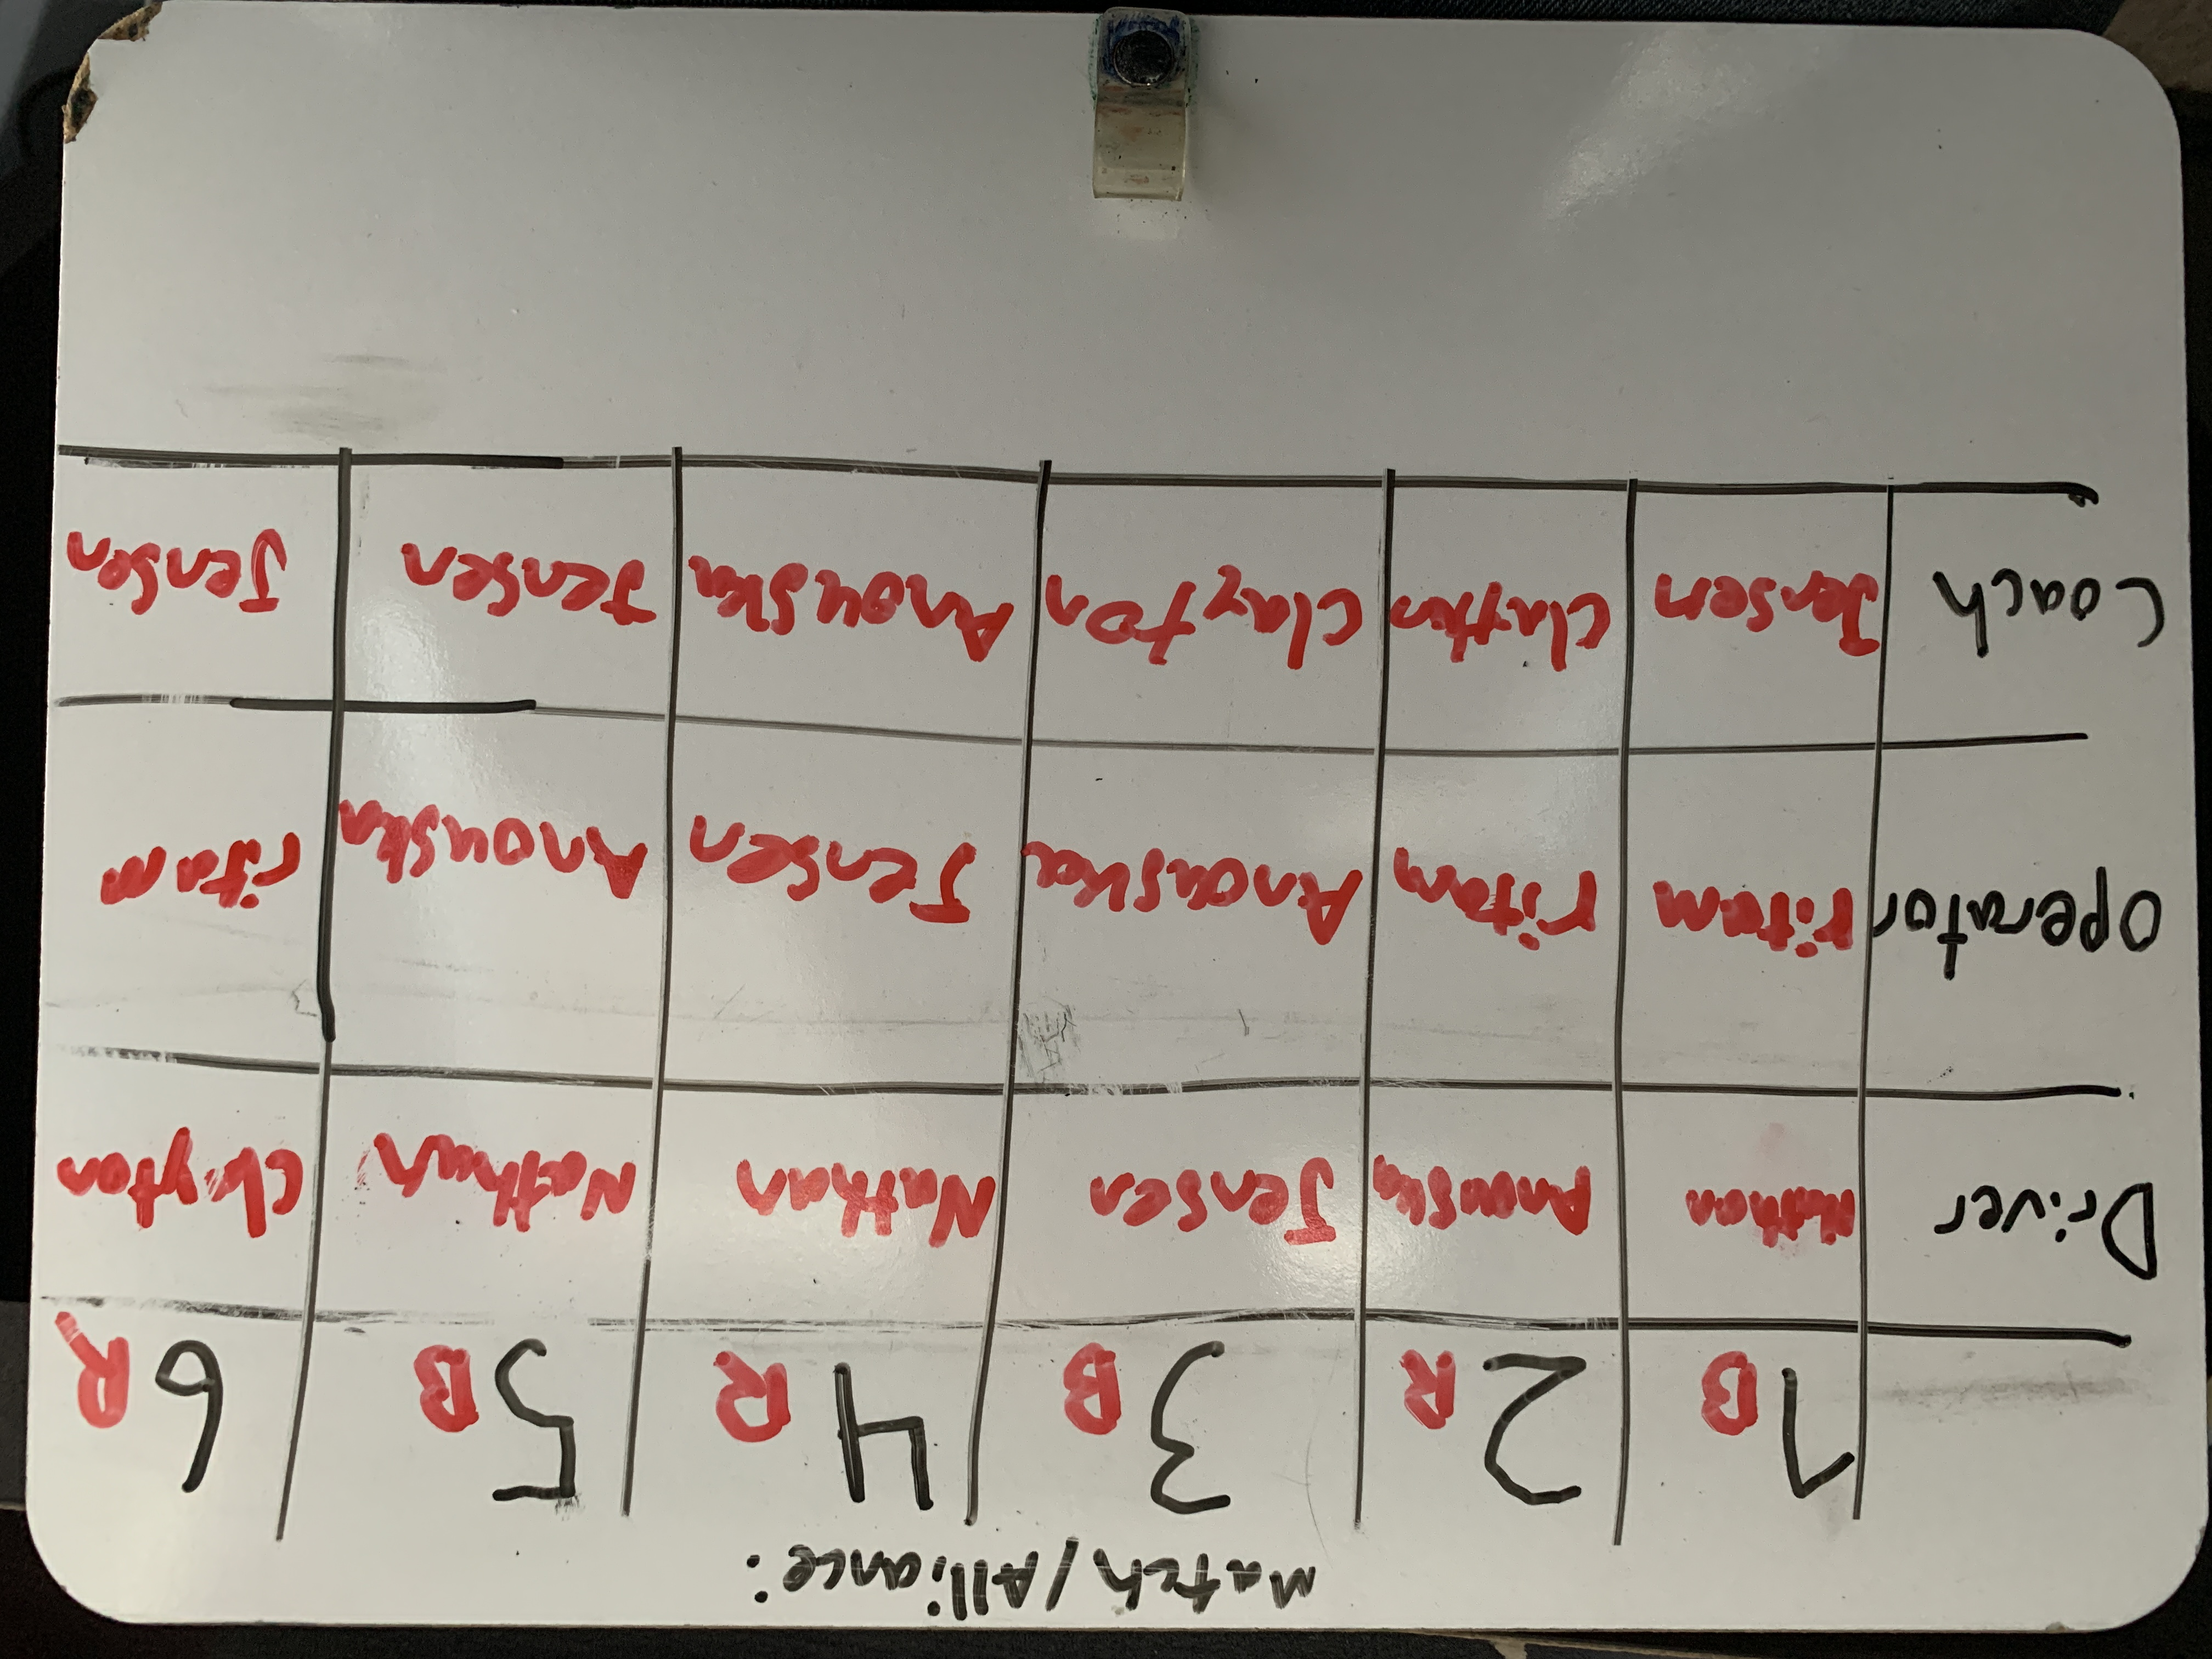
\includegraphics[width=0.95\textwidth]{Meetings/November/11-04-21/11-4-21_Team_Figure1 - Nathan Forrer.JPG}
  \caption{Our tryout schedule}
  \label{fig:pic1}
\end{minipage}%
\hfill%
\begin{minipage}[b]{.48\textwidth}
  \centering
  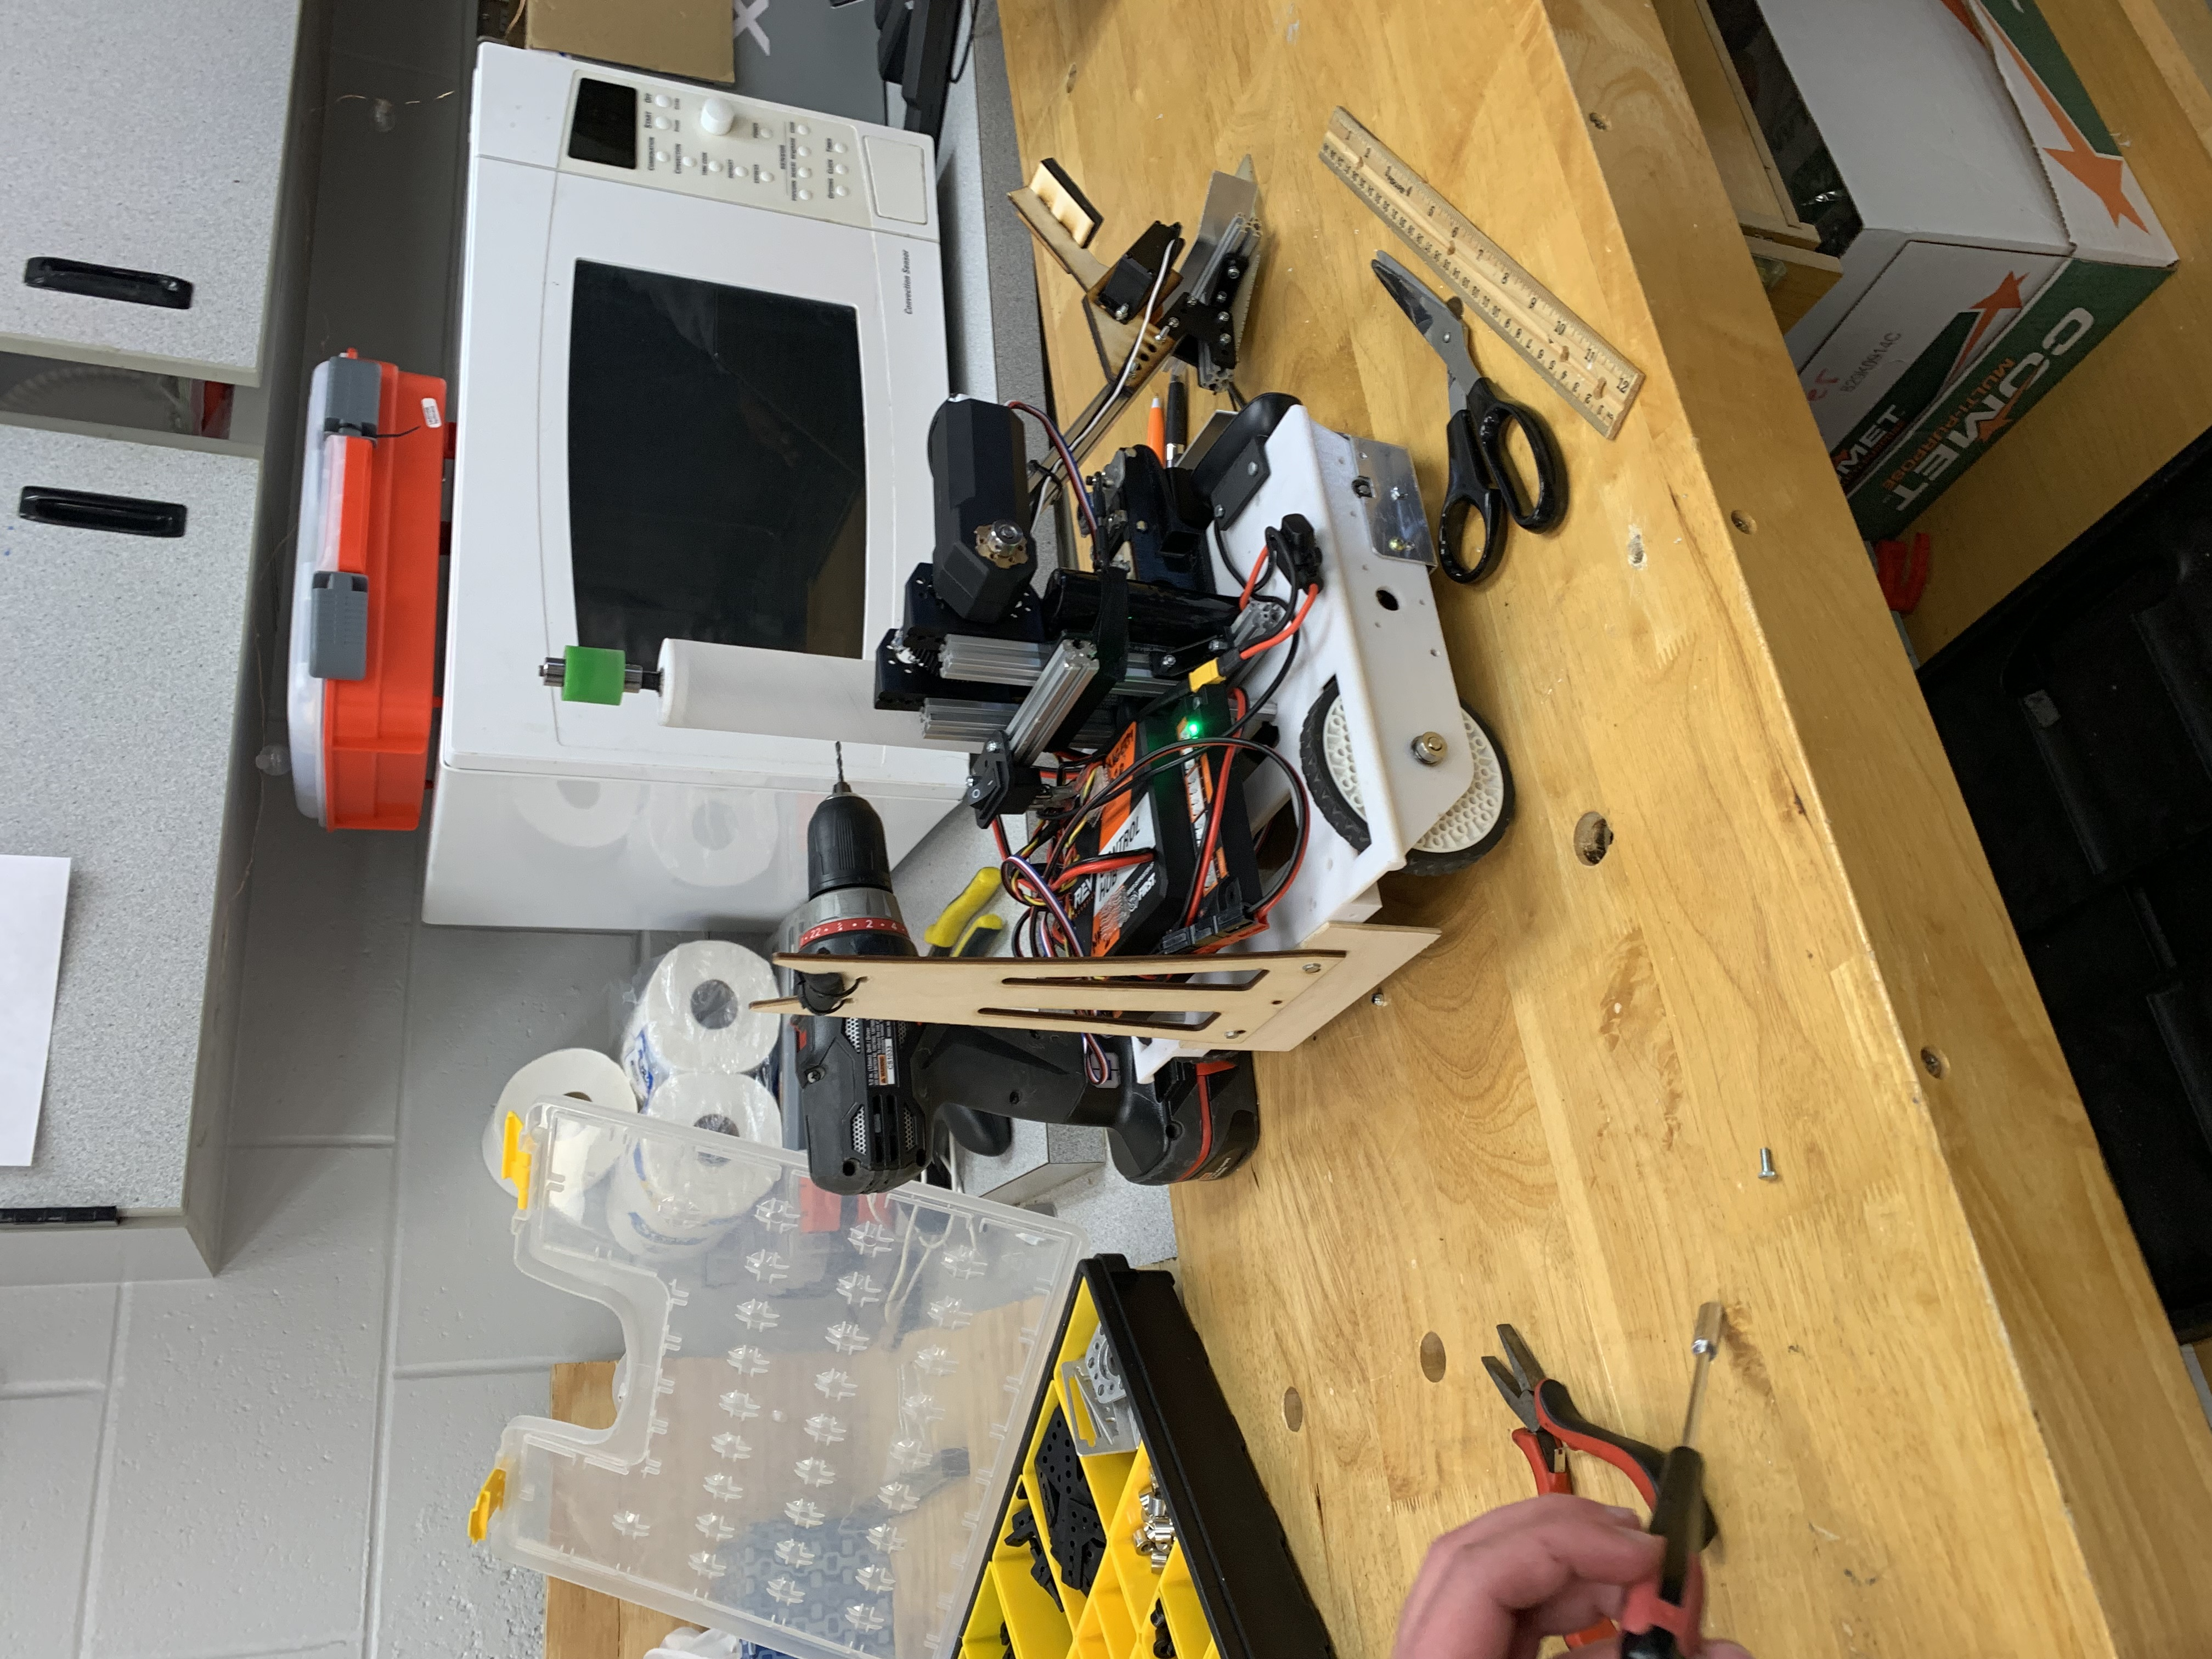
\includegraphics[width=0.95\textwidth]{Meetings/November/11-04-21/11-4-21_Team_Figure2 - Nathan Forrer.JPG}
  \caption{Robot ready for tryouts}
  \label{fig:pic2}
\end{minipage}
\end{figure}

\begin{figure}[htp]
\centering
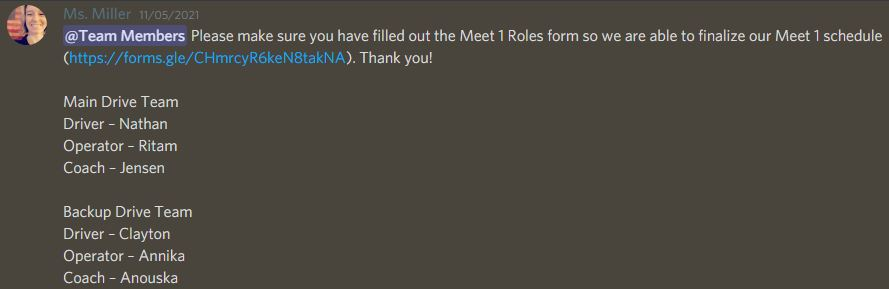
\includegraphics[width=0.95\textwidth, angle=0]{Meetings/November/11-04-21/11-4-21_Team_Figure3 - Nathan Forrer.JPG}
\caption{Meet 1 driveteam}
\label{fig:pic3}
\end{figure}


\whatsnext{
\begin{itemize}
    \item Work on autonomous
    \item Fix arm length
\end{itemize} 
}